В рамках НИР "Роль библиотек в эпоху искусственного интеллекта" центральной научной библиотеки Иркутского Института химии им. Е.А. Фаворсокого~\cite{refTrofimov}, опиряясь на результаты анализа предметной области и выявленные ограничения существующих подходов, разрабатывается программное обеспечение для оцифровки страниц химических книг. Функциональная логика системы и основные этапы обработки данных представлены на UML-диаграмме активностей~\cite{refUML} (рис.~\ref{fig:bisnes}).

\begin{figure*}[t]
	\centering
	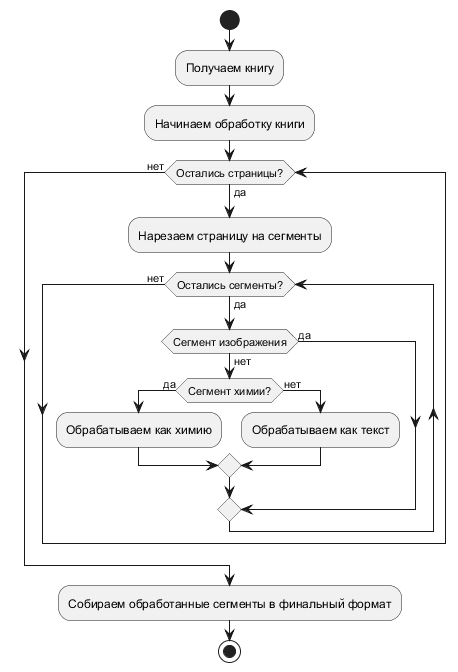
\includegraphics[width=0.55\linewidth]{img/chemistry_books_bisnes.png}
	\bicaption
	{UML-диаграмма активностей программы по обработке страниц книг по химии}
	{UML activity diagram of a program for processing pages of chemistry books}
	\label{fig:bisnes}
\end{figure*}

Программный комплекс реализован на языке Python, что объясняется его практической востребованностью в задачах обработки изображений и разработки интеллектуальных систем анализа документов. При проектировании использовались паттерны объектно-ориентированного проектирования~\cite{refGoF}, позволившие структурировать приложение и упростить его дальнейшее расширение. Для обеспечения единообразия и читаемости исходного кода соблюдались рекомендации Python Enhancement Proposals, в частности стандарты оформления кода PEP~8~\cite{refPEP8}.